\documentclass[12pt]{article}
\usepackage{amsmath}
\usepackage{amssymb}
\usepackage{graphicx}
\usepackage{geometry}
\geometry{margin=1in}

\title{Rigging Report}
\author{}
\date{\today}

\begin{document}

\maketitle

\section{Pipe Weight Calculation}
The weight of the spreader bar pipe is calculated as:
\[
\text{Weight per Meter} = \text{Outer Diameter} \times \pi \times \text{Thickness} \times 7.85
\]
\[
\text{Weight} = \text{Weight per Meter} \times \text{Length}
\]
The calculated weight of the spreader bar pipe is \textbf{2.28 T}.

\section{Position of Center of Gravity (C.O.G)}
\begin{center}
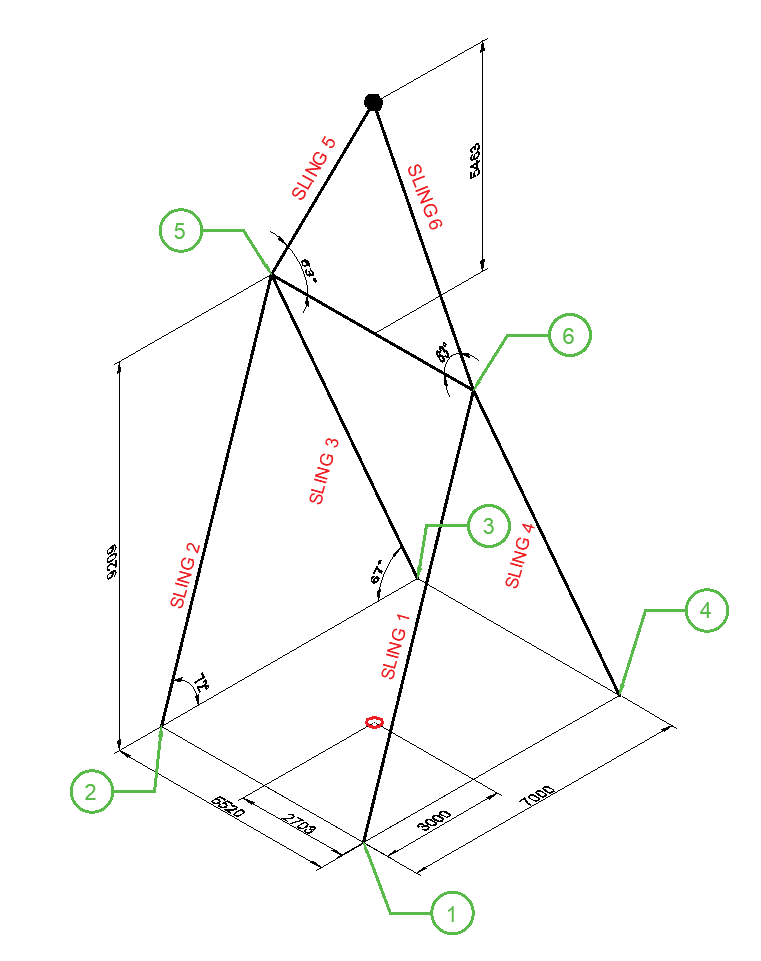
\includegraphics[width=0.6\textwidth]{image-3.png}
\end{center}
The position of the C.O.G is essential for stability. The distances from the C.O.G to each lifting point are used in the load calculations.

\section{Calculation for Each Lifting Point}
The load at each lifting point is calculated using (e.g., lifting point 1 and 2):
\[
L = W \times \left( \frac{d_{t1}}{od_{t1}} \right) \times \left( \frac{d_{t2}}{od_{t2}} \right)
\]
\begin{itemize}
  \item $L_1 = 150 \times \left( \frac{5520-2703}{5520} \right) \times \left( \frac{7000-3000}{7000} \right)$
  \item $L_2 = 150 \times \left( \frac{2703}{5520} \right) \times \left( \frac{7000-3000}{7000} \right)$
\end{itemize}

\begin{itemize}
  \item Lifting Point 1: 43.74 T
  \item Lifting Point 2: 41.97 T
  \item Lifting Point 3: 31.48 T
  \item Lifting Point 4: 32.81 T
  \item Lifting Point 5: 76.55 T
  \item Lifting Point 6: 73.45 T
\end{itemize}

\section{Tension Calculation}
The tension in each sling is:
\[
\text{Tension} = \frac{\text{Load}}{\sin(\theta)}
\]
\begin{itemize}
  \item Sling 1: 45.99 T (72$^\circ$)
  \item Sling 2: 44.13 T (72$^\circ$)
  \item Sling 3: 34.20 T (67$^\circ$)
  \item Sling 4: 35.64 T (67$^\circ$)
  \item Sling 5: 82.44 T (63$^\circ$)
  \item Sling 6: 85.91 T (63$^\circ$)
\end{itemize}

\section{Compressive Stress on the Spreader Bar}
The compressive stress is:
\[
\text{Longitudinal Load} = \text{Load} \times \cos(\theta)
\]
The total compressive stress on the spreader bar is \textbf{75.01 T}.

\section{Summary Tables}
\subsection*{Lifting Load at 4 Lifting Points and Padeye}
\begin{center}
\begin{tabular}{|c|c|}
\hline
Lifting Point & Load (T) \\
\hline
1 & 43.74 \\
2 & 41.97 \\
3 & 31.48 \\
4 & 32.81 \\
5 & 73.45 \\
6 & 76.55 \\
\hline
\end{tabular}
\end{center}

\subsection*{Tension of the Slings}
\begin{center}
\begin{tabular}{|c|c|c|}
\hline
Sling No. & Tension (T) & Angle ($^\circ$) \\
\hline
1 & 45.99 & 72 \\
2 & 44.13 & 72 \\
3 & 34.20 & 67 \\
4 & 35.64 & 67 \\
5 & 82.44 & 63 \\
6 & 85.91 & 63 \\
\hline
\end{tabular}
\end{center}

\subsection*{Compressive Stress on Spreader Bar}
\begin{center}
\begin{tabular}{|c|c|}
\hline
Component & Stress (T) \\
\hline
Total Compressive Stress & 75.01 \\
\hline
\end{tabular}
\end{center}

\end{document}
